\documentclass[10pt, a4paper]{article}
\usepackage[top=3cm, bottom=4cm, left=3.5cm, right=3.5cm]{geometry}
\usepackage{amsmath,amsthm,amsfonts,amssymb,amscd, fancyhdr, color, comment, graphicx, environ, pifont}
\usepackage{float}
\usepackage{mathrsfs}
\usepackage[math-style=ISO]{unicode-math}
\usepackage[framemethod=TikZ]{mdframed}
\usepackage{enumerate}
\usepackage[shortlabels]{enumitem}
\usepackage{fancyhdr}
\usepackage{indentfirst}
\usepackage{listings}
\usepackage{sectsty}
\usepackage{thmtools}
\usepackage{shadethm}
\usepackage{hyperref}
\usepackage{setspace}
\usepackage[linguistics]{forest}
\hypersetup{
    colorlinks=true,
    linkcolor=blue,
    filecolor=magenta,      
    urlcolor=blue,
}
\mdfsetup{skipabove=\topskip,skipbelow=\topskip}
\mdfdefinestyle{theoremstyle}{%
linecolor=black,linewidth=1pt,%
frametitlerule=true,%
frametitlebackgroundcolor=gray!20,
innertopmargin=\topskip,
}
\mdtheorem[style=theoremstyle]{Problem}{Problem}
\newenvironment{Solution}{\textbf{Solution.}}

\definecolor{codegreen}{rgb}{0,0.6,0}
\definecolor{codegray}{rgb}{0.5,0.5,0.5}
\definecolor{codepurple}{rgb}{0.58,0,0.82}
\definecolor{backcolour}{rgb}{0.95,0.95,0.92}

\lstdefinestyle{mystyle}{
    backgroundcolor=\color{backcolour},   
    commentstyle=\color{codegreen},
    keywordstyle=\color{magenta},
    numberstyle=\tiny\color{codegray},
    stringstyle=\color{codepurple},
    basicstyle=\ttfamily\footnotesize,
    breakatwhitespace=false,         
    breaklines=true,                 
    captionpos=b,                    
    keepspaces=true,                 
    numbers=left,                    
    numbersep=5pt,                  
    showspaces=false,                
    showstringspaces=false,
    showtabs=false,                  
    tabsize=2
}

\lstset{style=mystyle}
\newcommand{\norm}[1]{\left\lVert#1\right\rVert}     
\newcommand\course{Calculus and Applications}                            
\newcommand\hwnumber{MATH40003}                                  
\pagestyle{fancy}
\headheight 35pt
\lhead{\today}
\rhead{
\includegraphics[width=2.5cm]{icl_logo.png}}
\lfoot{}
\pagenumbering{arabic}
\cfoot{\small\thepage}
\rfoot{}
\headsep 1.2em
\renewcommand{\baselinestretch}{1.25}
\renewcommand{\labelenumi}{\alph{enumi})}
\newcommand{\Z}{\mathbb Z}
\newcommand{\R}{\mathbb R}
\newcommand{\Q}{\mathbb Q}
\newcommand{\NN}{\mathbb N}
\newcommand{\PP}{\mathbb P}
\DeclareMathOperator{\Mod}{Mod} 
\renewcommand\lstlistingname{Algorithm}
\renewcommand\lstlistlistingname{Algorithms}
\def\lstlistingautorefname{Alg.}
\newtheorem*{theorem}{Theorem}
\newtheorem*{lemma}{Lemma}
\newtheorem{case}{Case}
\newcommand{\assign}{:=}
\newcommand{\infixiff}{\text{ iff }}
\newcommand{\nobracket}{}
\newcommand{\backassign}{=:}
\newcommand{\tmmathbf}[1]{\ensuremath{\boldsymbol{#1}}}
\newcommand{\tmop}[1]{\ensuremath{\operatorname{#1}}}
\newcommand{\tmtextbf}[1]{\text{{\bfseries{#1}}}}
\newcommand{\tmtextit}[1]{\text{{\itshape{#1}}}}

\newenvironment{itemizedot}{\begin{itemize} \renewcommand{\labelitemi}{$\bullet$}\renewcommand{\labelitemii}{$\bullet$}\renewcommand{\labelitemiii}{$\bullet$}\renewcommand{\labelitemiv}{$\bullet$}}{\end{itemize}}
\catcode`\<=\active \def<{
\fontencoding{T1}\selectfont\symbol{60}\fontencoding{\encodingdefault}}
\catcode`\>=\active \def>{
\fontencoding{T1}\selectfont\symbol{62}\fontencoding{\encodingdefault}}
\catcode`\<=\active \def<{
\fontencoding{T1}\selectfont\symbol{60}\fontencoding{\encodingdefault}}
\begin{document}

\begin{titlepage}
    \begin{center}
        \vspace*{3cm}
            
        \Huge
        \textbf{
        Coursework}
            
            
        \vspace{1.5cm}
        \Large
            
        \textbf{
        CID number: There was a Mr. Number}% <-- author
        
            
        \vfill
        
    MATH40004 - Calculus and Applications - Term 2, 2023
        \vspace{1cm}
            
        
\includegraphics[width=0.4\textwidth]{icl_logo.png}
        \\
        
        \Large
        
        \today
            
    \end{center}
\end{titlepage}


\newpage
\begin{Problem}
\begin{enumerate}
  \item Consider the following system of differential equations:
\end{enumerate}

$$
\frac{d}{d t}\left(\begin{array}{l}
x \\
y
\end{array}\right)=\left(\begin{array}{ll}
1 & -2 \\
3 & -3
\end{array}\right)\left(\begin{array}{l}
x \\
y
\end{array}\right) .
$$

(a) Find the solution for this system in terms of real functions.

(b) Sketch the phase portrait for this system in the phase plane. Describe the asymptotic behavior explaining your reasoning.

(c) Find $\gamma$ and $\omega$ such that the equation

$$
\frac{d^{2} x}{d t^{2}}+\gamma \frac{d x}{d t}+\omega^{2} x=0
$$

has the same dynamics as the system (1).

(d) Consider now the system:

$$
\frac{d}{d t}\left(\begin{array}{l}
x \\
y
\end{array}\right)=\left(\begin{array}{cc}
1 & -2 \\
3 & -3+\epsilon
\end{array}\right)\left(\begin{array}{l}
x \\
y
\end{array}\right) .
$$

Using a graph of $\tau$ and Delta plane, find the value of $\epsilon \in \mathbb{R}$ at which the system undergoes a bifurcation (where the system changes stability).

(e) Finally consider the non-homogenous system:

$$
\frac{d}{d t}\left(\begin{array}{l}
x \\
y
\end{array}\right)=\left(\begin{array}{ll}
1 & -2 \\
3 & -3
\end{array}\right)\left(\begin{array}{l}
x \\
y
\end{array}\right)+\left(\begin{array}{c}
e^{-t} \\
0
\end{array}\right) .
$$

Find the general solution and particularize it when $x(0)=1$ and $y(0)=0$.

\end{Problem}
\begin{Solution}
\begin{enumerate}
    \item{(a)}
    We set
    \begin{equation*}
        \mathbf{A}=
        \begin{bmatrix}
            1 & -2 \\
            3 & -3
        \end{bmatrix}
    \end{equation*}
        Then, we try to find the eigenvalues of $\mathbf{A}$.
        \begin{align*}
            \det (\mathbf{A}-\lambda \mathbf{I})&=0\\
            \lambda^{2}+2 \lambda+3&=0\\
            (\lambda+1)^2&=-2\\
            \lambda_1&=-1+i\sqrt{2}\\
            \lambda_2&=-1-i\sqrt{2}
        \end{align*}
        Then, we find the eigenvectors of $\mathbf{A}$.For $\lambda_1 = -1+i\sqrt{2}$, we have
        \begin{equation*}
           \begin{bmatrix}
            2- i\sqrt{2} & -2 \\
            3 & -2- i\sqrt{2}
           \end{bmatrix}
           \begin{bmatrix}
            x\\
            y
           \end{bmatrix}
           =0
        \end{equation*}
        We solve this system to get
        \begin{equation*}
            \left\{ \begin{array}{lr}
                x = 2\\
                y = 2 - i\sqrt{2}
            \end{array}
                \right.
            \end{equation*}
            Therefore, the eigenvector is
            \begin{equation*}
                \vec {v_1} = \begin{bmatrix}
                    2\\
                    2 - i\sqrt{2}
                \end{bmatrix}
            \end{equation*}
            For $\lambda_2 = -1-i\sqrt{2}$, we have
        \begin{equation*}
           \begin{bmatrix}
            2+ i\sqrt{2} & -2 \\
            3 & -2+ i\sqrt{2}
           \end{bmatrix}
           \begin{bmatrix}
            x\\
            y
           \end{bmatrix}
           =0
        \end{equation*}
        We solve this system to get
        \begin{equation*}
            \left\{ \begin{array}{lr}
                x = 2\\
                y = 2 +i\sqrt{2}
            \end{array}
                \right.
            \end{equation*}
            Therefore, the eigenvector is
            \begin{equation*}
                \vec {v_2} = \begin{bmatrix}
                    2\\
                    2 + i\sqrt{2}
                \end{bmatrix}
            \end{equation*}
            So, we have the general solution of the system
            \begin{align*}
                \begin{bmatrix}
                    x\\
                    y
                \end{bmatrix}
                =c_1e^{t(-1+i\sqrt{2})}\begin{bmatrix}
                    2\\
                    2 - i\sqrt{2}
                \end{bmatrix}
                +c_2e^{t(-1-i\sqrt{2})}\begin{bmatrix}
                    2\\
                    2 + i\sqrt{2}
                \end{bmatrix}\\
                \begin{bmatrix}
                    x\\
                    y
                \end{bmatrix}
                =e^{-t}\left(c_1e^{i \sqrt{2} t}\begin{bmatrix}
                    2\\
                    2 - i\sqrt{2}
                \end{bmatrix}
                +c_2e^{-i \sqrt{2} t}\begin{bmatrix}
                    2\\
                    2 + i\sqrt{2}
                    \end{bmatrix}\right)
            \end{align*}
            We use the Eurler's formula to get
            \begin{equation*}
                \begin{bmatrix}
                    x\\
                    y
                \end{bmatrix}
                =e^{-t}\left((c_1+c_2)\begin{bmatrix}
                    2\cos(\sqrt{2}t)\\
                    2\cos(\sqrt{2}t)+\sqrt{2}\sin(\sqrt{2}t)
                \end{bmatrix}+
                i(c_1-c_2)\begin{bmatrix}
                    2\sin(\sqrt{2}t)\\
                    2\sin(\sqrt{2}t)-\sqrt{2}\cos(\sqrt{2}t)
                \end{bmatrix}\right)
            \end{equation*}
            We define $A_1 = c_1+c_2$ and $A_2 = i(c_1-c_2)$ as new real constants of integration, we can write the general solution as
            \begin{equation*}
                \begin{bmatrix}
                    x\\
                    y
                \end{bmatrix}
                =A_1 e^{-1}\begin{bmatrix}
                    2\cos(\sqrt{2}t)\\
                    2\cos(\sqrt{2}t)+\sqrt{2}\sin(\sqrt{2}t)
                \end{bmatrix}+
                A_2 e^{-1} \begin{bmatrix}
                    2\sin(\sqrt{2}t)\\
                    2\sin(\sqrt{2}t)-\sqrt{2}\cos(\sqrt{2}t)
                \end{bmatrix}
            \end{equation*}
            \newpage
            \item [(b)]
                 This is the phase portrait of this system that I drew using Python.\\
                   \begin{center}
                    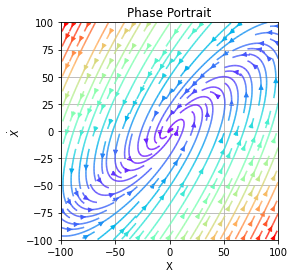
\includegraphics[scale=0.7]{output.png}
                   \end{center}
                This is the phase portrait of this system that I drew by hand.
                \begin{center}
                    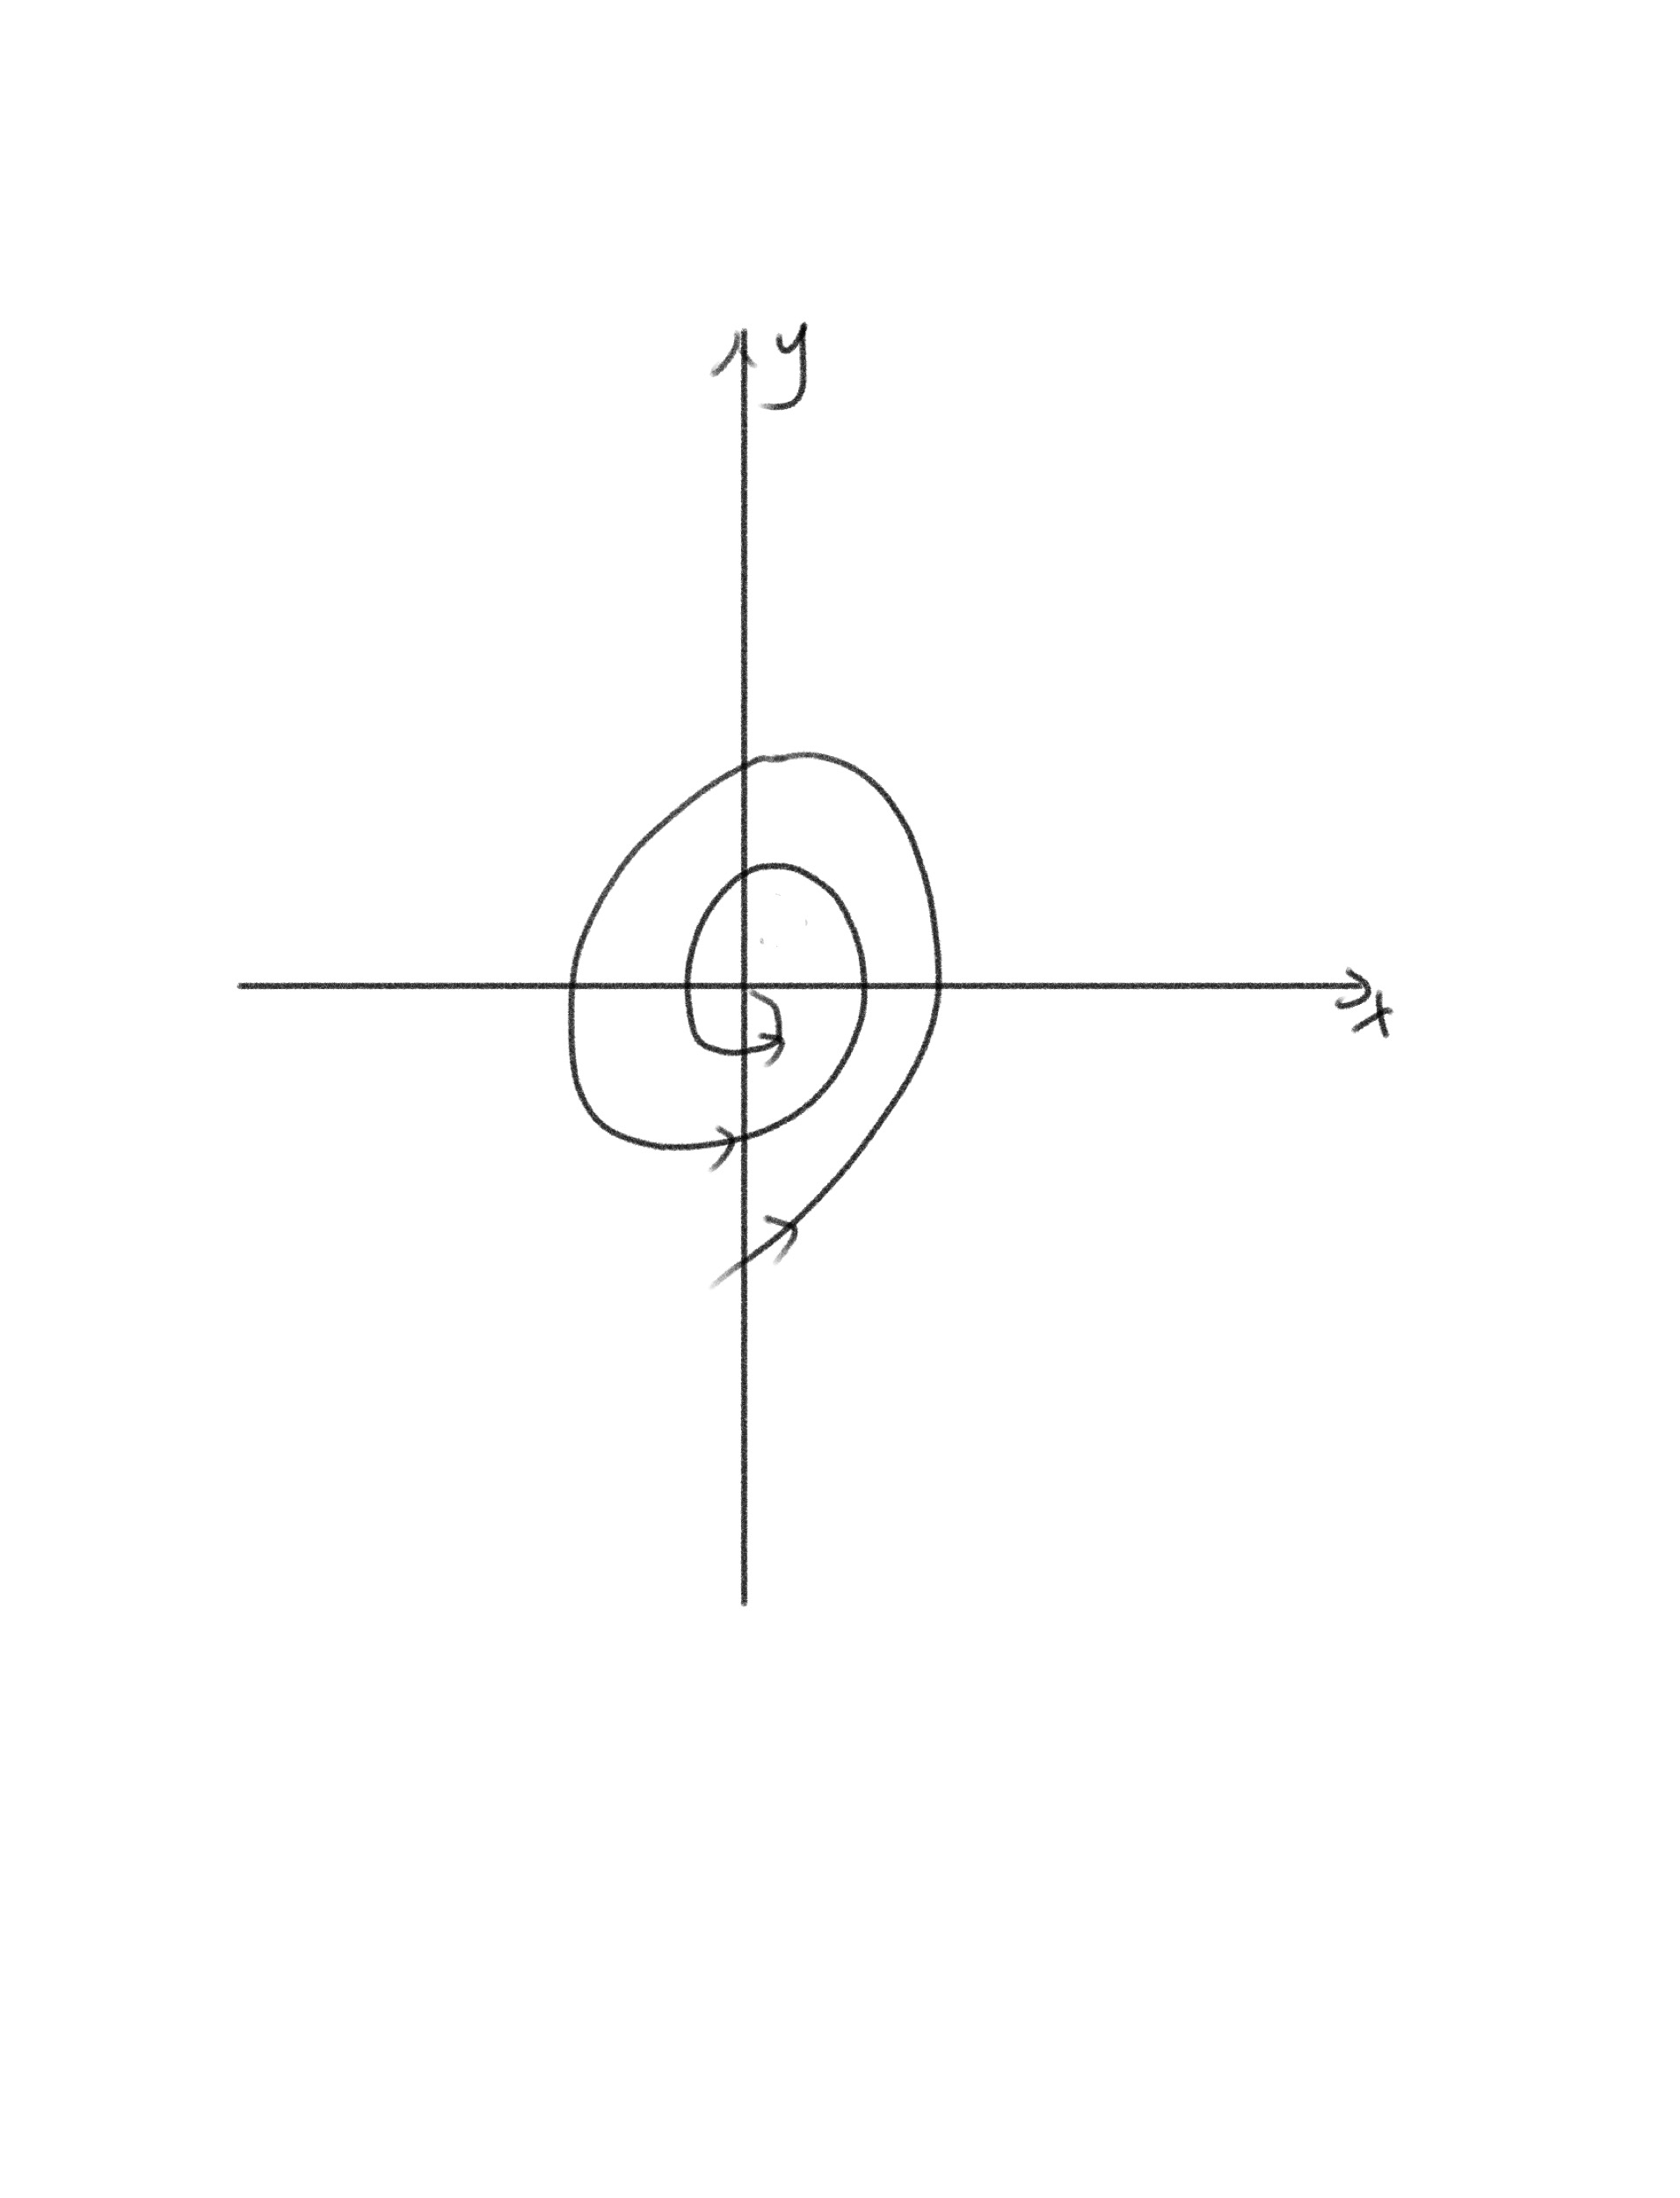
\includegraphics[scale=0.15]{Note 14 Mar 2023 at 02_12_15.jpg}
                \end{center}
                The asymptotic behavior of the solution is that the solution will converge to the point $(0,0)$.
                which, asymptotically as $ t \to \infty, \; 
                \begin{bmatrix}
                    x\\
                    y
                \end{bmatrix}  \to 
                \begin{bmatrix}
                    0\\
                    0
                \end{bmatrix}$.
                Since the eigenvalues are complex with the real part being negative, the solution will converge to the origin as $t$ become larger. Besides, by the phase portrait that we drew, this is an inward spiral and the fixed point is asymptomatically stable.
                \item[(c)]
                     Since
                     $$
                     \mathbf{A} = 
                     \begin{bmatrix}
                        2 & -2 \\
                        3 & -2
                    \end{bmatrix}
                    $$ by the definition of the trace and the determinant of $\mathbf{A}$, we have
                    \begin{equation*}
                            \tau = \text{trace}(\mathbf{A}) = 1-(-3) = 2 \quad
                            \Delta=\text{Det}(\mathbf{A}) = -3+6 = 3
                    \end{equation*}
                    For equation
                    \begin{equation*}
                        \frac{d^{2} x}{d t^{2}}+\gamma \frac{d x}{d t}+\omega^{2} x=0
                    \end{equation*}
                    We set $u = \frac{dx}{dt}$, then we get
                    \begin{equation*}
                        \frac{d^{2} x}{d t^{2}}+\gamma \frac{d x}{d t}+\omega^{2} x=0
                        \Leftrightarrow
                        \frac{du}{dt}+\gamma u+\omega^{2} x=0
                    \end{equation*}
                    Then we get the system of first order differential equations,
                    \begin{equation*}
                        \left\{
                            \begin{array}{lr}
                                \frac{dx}{dt} = u\\
                                \frac{du}{dt} = -\gamma u-\omega^{2} x
                            \end{array}
                            \right.
                    \end{equation*}
                    which is equivalent to the system of first order differential equations
                    \begin{equation*}
                        \frac{d}{dt}\begin{bmatrix}
                            x\\
                            u
                        \end{bmatrix} =
                        \begin{bmatrix}
                            0 & 1\\
                            -\omega^{2} & -\gamma
                        \end{bmatrix}
                        \begin{bmatrix}
                            x\\
                            u
                        \end{bmatrix}
                    \end{equation*}
                    The trace and the determinant of the matrix $\begin{bmatrix}
                            0 & 1\\
                            -\omega^{2} & -\gamma
                        \end{bmatrix}$ are
                        \begin{equation*}
                            \tau = -\gamma \quad
                            \Delta= \omega^{2}
                        \end{equation*}
                        We require that the equation must have the same dynmaics as the system $(1)$, so we have
                        \begin{equation*}
                            \gamma = -2 \quad
                            \omega^2 = 3
                        \end{equation*}
                        which means that 
                        \begin{equation*}
                            \gamma = -2 \quad
                            \omega = \pm \sqrt{3}
                        \end{equation*}
                        then, the two equations have the same dynamics.
                        \item [(d)] For the system, we have
                        \begin{equation*}
                            \tau = -2+\epsilon \quad
                            \Delta= 3+\epsilon
                        \end{equation*}
                        so $\tau$ and $\Delta$ both depend on the tuneble parameter $\epsilon$.
                        then, we have
                        \begin{equation*}
                            \Delta = \tau +5
                        \end{equation*}
                        \begin{center}
                            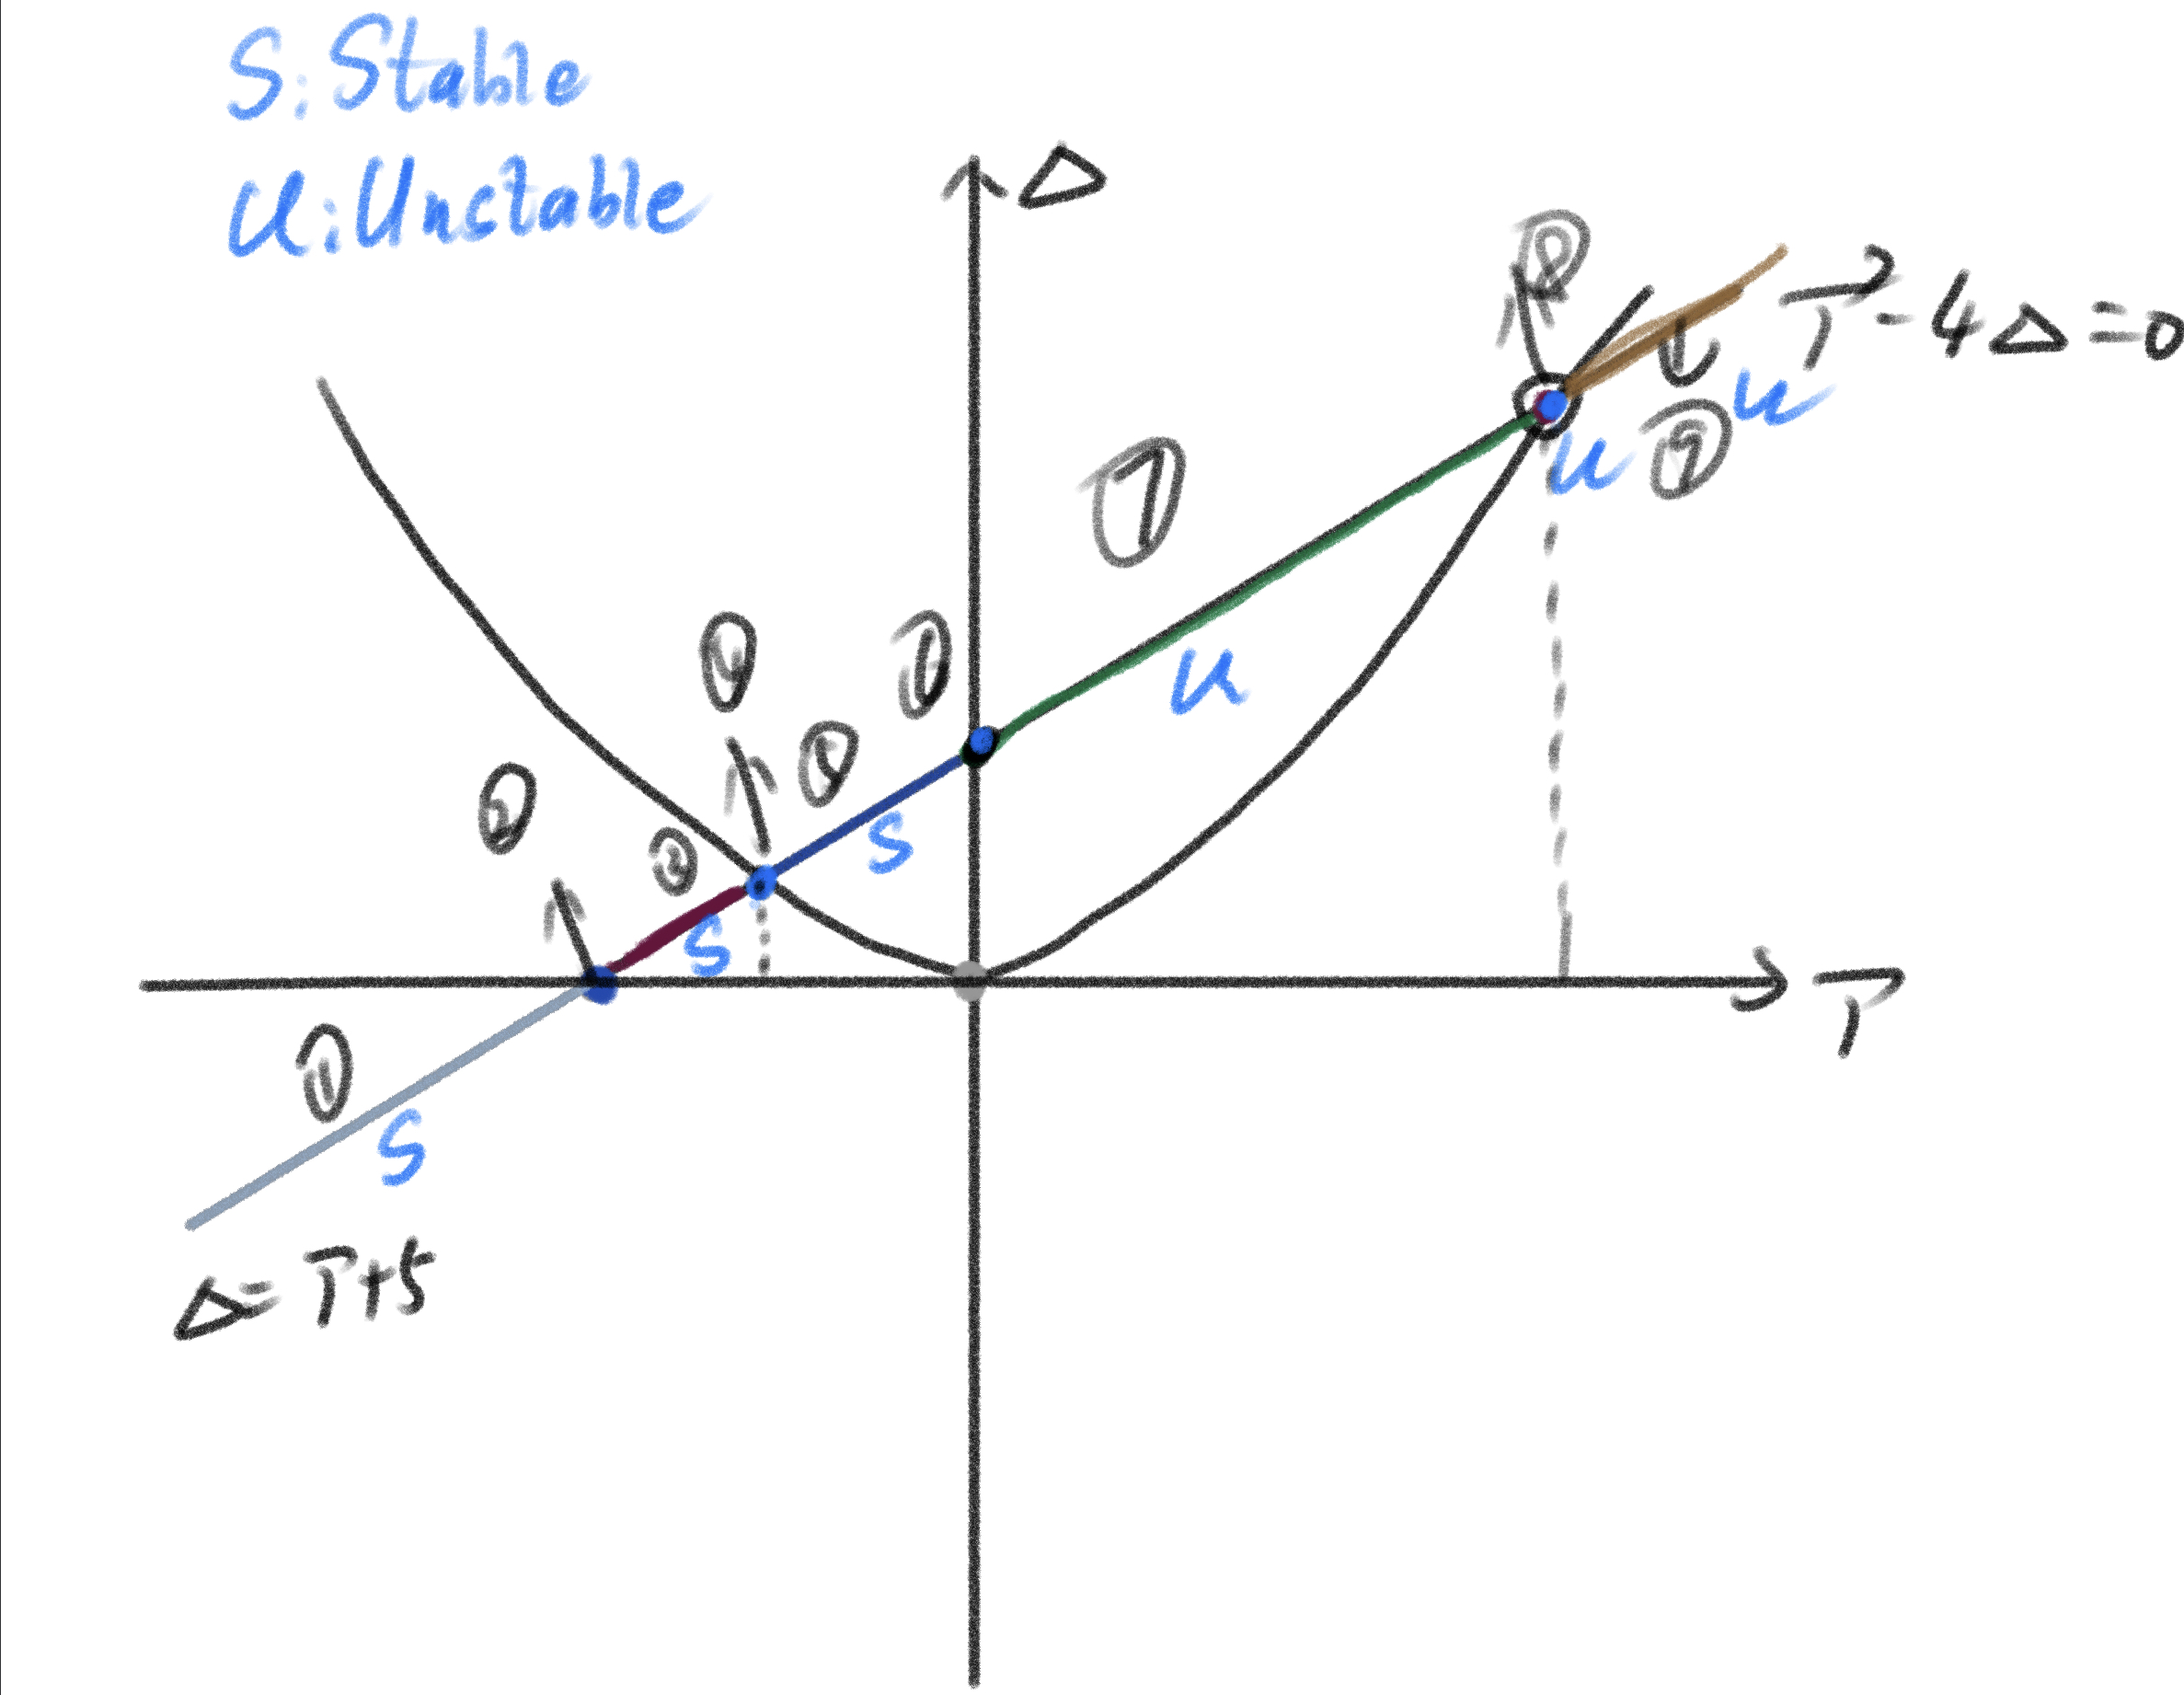
\includegraphics[scale=0.17]{IMG_0454.jpg} 
                        \end{center}
                        This is the $\tau$ and $\Delta$ plane. There are $9$ different qualitative behavior, as we vary $\epsilon $. At $\tau = 0$, we have a bifurcation as we go from region $5$ that is assmptotically  stable to the point $6$ that is Lyapanov stable and region $7$ that is unstable. 
                        \begin{align*}
                            \tau = -2 + \epsilon &= 0\\
                            \epsilon &= 2
                        \end{align*}
                        Therefore, when $\epsilon = 2$, the system undergoes a bifurcation.
                        \item[(e)] From $(a)$, we know that the general solution to the corresponding homogenous system is
                        \begin{equation*}
                            \begin{bmatrix}
                                x\\
                                y
                            \end{bmatrix}
                            =A_1 e^{-1}\begin{bmatrix}
                                2\cos(\sqrt{2}t)\\
                                2\cos(\sqrt{2}t)+\sqrt{2}\sin(\sqrt{2}t)
                            \end{bmatrix}+
                            A_2 e^{-1} \begin{bmatrix}
                                2\sin(\sqrt{2}t)\\
                                2\sin(\sqrt{2}t)-\sqrt{2}\cos(\sqrt{2}t)
                            \end{bmatrix}
                        \end{equation*}
                            Then, we try to find a particular integral solution to the corresponding non-homogenous system. We try to use the ansatz with the form
                            \begin{equation*}
                                \begin{bmatrix}
                                    A e^{-t}\\
                                    B e^{-t}    
                                \end{bmatrix}
                            \end{equation*} with $A$ and $B$ are constants to be determined.
                            Then, we get
                            \begin{equation*}
                                \frac{d}{dt} \begin{bmatrix}
                                    A e^{-t}\\
                                    B e^{-t}    
                                \end{bmatrix} - 
                                \begin{bmatrix}
                                    1 & -2 \\
                                    3 & -3
                                \end{bmatrix}
                                \begin{bmatrix}
                                    A e^{-t}\\
                                    B e^{-t}
                                \end{bmatrix}
                                = \begin{bmatrix}
                                    e^{-t}\\
                                    0
                                \end{bmatrix}
                            \end{equation*}
                            which is equivalent to
                            \begin{equation*}
                                \left\{ \begin{array}{lr}
                                    -A e^{-t} -A e^{-t} + 2B e^{-t} = e^{-t}\\
                                    -B e^{-t} - 3A e^{-t} + 3B e^{-t} = 0
                                \end{array}
                                    \right.
                            \end{equation*}
                            $$ \Downarrow $$
                            \begin{equation*}
                                \left\{ \begin{array}{lr}
                                   A = 1\\
                                   B = \frac{3}{2}
                                \end{array}
                                    \right.
                            \end{equation*}
                            Then, the particular integral solution is
                            \begin{equation*}
                                \begin{bmatrix}
                                    e^{-t}\\
                                    \frac{3}{2} e^{-t}
                                \end{bmatrix}
                            \end{equation*}
                            Hence, the general solution is
                            \begin{equation*}
                                \begin{bmatrix}
                                    x\\
                                    y
                                \end{bmatrix}
                                =A_1 e^{-1}\begin{bmatrix}
                                    2\cos(\sqrt{2}t)\\
                                    2\cos(\sqrt{2}t)+\sqrt{2}\sin(\sqrt{2}t)
                                \end{bmatrix}+
                                A_2 e^{-1} \begin{bmatrix}
                                    2\sin(\sqrt{2}t)\\
                                    2\sin(\sqrt{2}t)-\sqrt{2}\cos(\sqrt{2}t)
                                \end{bmatrix}+
                                \begin{bmatrix}
                                    e^{-t}\\
                                    \frac{3}{2} e^{-t}
                                \end{bmatrix}
                            \end{equation*}
                            Since, $x(0)=1$ and $y(0)=0$, we have
                            \begin{equation*}
                                \begin{bmatrix}
                                    1\\
                                    0
                                \end{bmatrix}
                                =A_1 e^{-1}\begin{bmatrix}
                                    2\\
                                    2
                                \end{bmatrix}+
                                A_2 e^{-1} \begin{bmatrix}
                                    0\\
                                    -\sqrt{2}
                                \end{bmatrix}+
                                \begin{bmatrix}
                                    1\\
                                    \frac{3}{2} 
                                \end{bmatrix}
                            \end{equation*}
                            which is equivalent to
                            \begin{equation*}
                                \left\{ \begin{array}{lr}
                                    2A_1 e^{-1}+1 = 1\\
                                    2A_1 e^{-1} - \sqrt{2}A_2 e^{-1} + \frac{3}{2}= 0\\
                                \end{array}
                                    \right.
                            \end{equation*}
                            $$ \Downarrow $$
                            \begin{equation*}
                                \left\{ \begin{array}{lr}
                                   A_1 = 0\\
                                   A_2 = \frac{3\sqrt{2}}{4}e
                                \end{array}
                                    \right.
                            \end{equation*}
                            Therefore, the particular solution with $x(0)=1$ and $y(0)=0$ is
                            \begin{equation*}
                                \begin{bmatrix}
                                    x\\
                                    y
                                \end{bmatrix}
                                =\frac{3\sqrt{2}}{4} \begin{bmatrix}
                                    2\sin(\sqrt{2}t)\\
                                    2\sin(\sqrt{2}t)-\sqrt{2}\cos(\sqrt{2}t)
                                \end{bmatrix}+
                                \begin{bmatrix}
                                    e^{-t}\\
                                    \frac{3}{2} e^{-t}
                                \end{bmatrix}
                            \end{equation*} 

\end{enumerate}
\end{Solution}
\end{document}
